\documentclass{llncs}
\let\algorithm\relax
\let\endalgorithm\relax

\usepackage{epsfig,amsmath,amssymb,graphicx,algorithmic,multirow,listings,url,color,verbatim,moreverb,eurosym,booktabs,setspace,algorithm,caption, subcaption}
\usepackage[english]{babel}
\usepackage[utf8]{inputenc}


\usepackage[usenames,dvipsnames]{xcolor}
\usepackage[font=small,labelfont=bf,hypcap,labelsep=period]{caption}
\usepackage{hyperref}
\hypersetup{colorlinks=true, citecolor=Blue, linkcolor=OrangeRed, bookmarksnumbered=true}
\graphicspath{{./figures/},{./}}

\newcommand{\mc}[3]{\multicolumn{#1}{#2}{#3}}
\newcommand{\mr}[2]{\multirow{#1}{*}{#2}}

\definecolor{listinggray}{gray}{0.9}

\clubpenalty = 10000
\widowpenalty = 10000
\displaywidowpenalty = 10000


\usepackage{dcolumn}
\newcolumntype{d}{D{.}{.}{2,7}}
\newcolumntype{b}{D{.}{.}{2,6}}
\newcolumntype{m}{D{m}{}{2,6}}



\begin{document}
\def\Fnospace~{Fig.{}}
\def\Anospace~{Alg.{}}
\def\sectionautorefname{Section}
\def\subsectionautorefname{Subsection}
\def\figureautorefname{\Fnospace~}
\def\algorithmautorefname{\Anospace~}

\mainmatter  % start of an individual contribution

\title{Detection of Multiple Implicit Features per Sentence in Consumer Review Data}
\author{Nikoleta Dosoula \and Roel Griep \and Rick den Ridder \and Rick Slangen \and \\Kim Schouten \and Flavius Frasincar}
\titlerunning{Detection of Multiple Implicit Features per Sentence in Consumer Review Data}
\authorrunning{N. Dosoula et al.}
\institute{Erasmus University Rotterdam\\ PO Box 1738, NL-3000 DR\\ Rotterdam, the Netherlands\\
 \email{\{384964nd,416133rg,324065rr,362941rs\}@student.eur.nl, \{schouten,frasincar\}@ese.eur.nl}
}

\toctitle{Detection of Multiple Implicit Features per Sentence in Consumer Review Data}
\tocauthor{Nikoleta Dosoula, Roel Griep, Rick den Ridder, Rick Slangen, Kim Schouten, and Flavius Frasincar}
\maketitle


\begin{abstract}
With the rise of e-commerce, online consumer reviews have become crucial for consumers' purchasing decisions. Most of the existing research focuses on the detection of explicit features and sentiments in such reviews, thereby ignoring all that is reviewed \textit{implicitly}.
%Although research is shifting its focus towards extracting implicit features, some methods are designed to find only one implicit feature assignment per sentence. This approach is, however, unrealistically constrained and results in loss of information. Diagnosing this shortcoming,
This study builds, in extension of an existing implicit feature algorithm that can only assign one implicit feature to each sentence, a classifier that predicts the presence of multiple implicit features in sentences. The classifier makes its prediction based on a score function and is trained by means of a threshold. Only if this score exceeds the threshold, we allow for the detection of multiple implicit feature. In this way, we increase the recall while limiting the decrease in precision. In the more realistic scenario, the classifier-based approach improves the $F_1$-score by 1.6 percentage points on a restaurant review data set.
\keywords{Feature detection $\cdot$ Aspect category detection $\cdot$ Sentiment analysis $\cdot$ Aspect level sentiment analysis}
\end{abstract}


\section{Introduction} \label{sec:intro}
	In the last decade, a growing amount of retail activity is transferred from the street to the Web. Nowadays, people buy a wide range of consumer goods online using websites such as Amazon or Alibaba. These e-commerce companies often provide an easily accessible platform where consumers can share their experiences with and opinions about their purchases in the form of product reviews. As the required effort for writing these reviews becomes increasingly little, the number of product reviews on online retail shops sharply increased during the last decade. To illustrate this, in 2014 the number of reviews on Amazon exceeded the 10 million~\cite{FFACF2014}. Furthermore, the number of online reviewing platforms, where consumers leave behind product or service reviews, continues to grow.
	
	Using these product reviews for decision making has become increasingly popular~\cite{SN2004}. Where some consumers might be looking for specific comments on their potential purchase, others might only be interested in the overall sentiment or in the sentiment per product aspect.  However, the number of reviews can be high for some (popular) products, which makes reading all those reviews very time consuming. In order to lower these information costs, one of three pillars in the classical transaction cost model~\cite{D1979}, an automatic assessment of the overall sentiment within consumer reviews is asked for.
	
	%Whereas much of the existing literature is concerned with determining  the overall sentiment within product reviews, \cite{SF2014} brings attention to the classification of the sentiment per product feature.
	%A vital step to realize this, is to automatically connect so-called \textit{sentiment words}, such as `good', `delicious', or `overestimated', with \textit{product features}, such as `price', `quality', and `energy usage'. By this manner, sentiments per product feature can be automatically determined based on written consumer reviews. However, the detection of such links between the sentiment and the feature in each sentence can be difficult, especially when the feature itself is not explicitly mentioned.
	
	%For the sake of illustration, we take two sentences from data set, consisting of a collection of restaurants reviews concerning one (or more) of five features of the restaurant:
	%\begin{quote}
	%\emph{Review 1:} ``It's a perfect place to have amazing Indian food.''\\
	%\emph{Review 2:} ``The fried rice is amazing here.''
	%\end{quote}
	
	%In the first review, the words `amazing' and `food' are explicitly mentioned and could therefore be relatively easily detected and linked. In contrast, the second review does not explicitly mention the feature `food'. Nonetheless, the reader could infer that the writer comments on the quality  of the food that was served in the restaurant, which is the \textit{implicit feature} in this sentence. \cite{SF2014} argues that the group of features to which consumer often implicitly refer, generally contains a number of features that are of high relative importance. The reasons for this is that for humans to infer implicit features from sentences, there needs to be a shared understanding between the writer and the reader about the relation between the actual words in the sentence and the implied feature. In general, writers of reviews can only rely on this shared understanding when writing about well-known features. Not being able to include this group of features in a typical sentiment analysis is likely to be harmful to a feature-based sentiment analysis. As such, the detection of these implicit features plays a key role in the classification of sentiment per product feature.
	
	The main aim of this paper is to contribute to the existing research on the detection of implicit features within consumer reviews. In particular, we seek to extend the method proposed in~\cite{SF2014} by adding a classifier that predicts the presence of multiple implicit features within a sentence. The evaluation of our method shows that we can significantly improve the $F_1$-measure by 1.6\% compared to~\cite{SF2014}, resulting in an $F_1$-measure equal to 64.5\%. Apart from increasing the $F_1$-measure, our method contributes to existing work by its suitability for a more realistic scenario in which sentences are allowed to have more than one implicit feature.
	
	The remaining part of this paper is organized as follows. Sect.~\ref{sec:relWork} reviews the relating literature and addresses the possible shortcomings of previously proposed methods. After presenting our method in Sect.~\ref{sec:meth}, we discuss the data set used in our experiments in Sect.~\ref{sec:data}. Sect.~\ref{sec:impl} then discusses the implementation of our proposed method and we evaluate its performance in Sect.~\ref{sec:eval}, also by comparing it to previous work in the literature. Sect.~\ref{sec:conc} concludes this paper and proposes possible avenues for future research.

\section{Related Work}\label{sec:relWork}
	This section discusses the relevant literature in the field that is concerned with the automated assignment of implicit product features within consumer reviews. Our proposed method is motivated by the shortcomings of existing approaches. %The first part of this section addresses some of the most relevant implicit feature extraction methods previously proposed in literature. The second part particularly focuses on how to handle the presence of multiple implicit features within one sentence.
	
	%\subsection{Implicit feature extraction}\label{sec:featextr}
	The vast majority of approaches in the literature focuses on finding the explicit features in sentences. This limited approach is understandable because often in reviews most of the features are explicitly mentioned in a sentence. However, as addressed before, features that are implicitly mentioned in reviews are equally important. In feature-based sentiment analysis the detection of implicit feature therefore plays an essential role. However, in order to obtain reliable results, sophisticated methods that can infer implicit features from sentences are required. This section addresses some of the most relevant approaches.
	
	A method of detecting implicit features is proposed in~\cite{HCK2011}. More specifically, the method refers to a two-phase co-occurrence association rule mining approach. In the first phase,~\cite{HCK2011} mines a set of association rules from co-occurrences between opinion words and explicit features. Therefore each opinion word is associated with a set of candidate features. In the second phase, the explicit features are clustered in order to obtain more powerful rules. If an opinion word is not linked with an explicit feature, the list of rules is checked in order to assign the most likely feature to this opinion word.
	% In this paper, we propose a novel two-phase co-occurrence association rule mining approach to identifying implicit features. Specifically, in the first phase of rule generation, for each opinion word occurring in an explicit sentence in the corpus, we mine a significant set of association rules of the form [opinion-word, explicit-feature] from a co-occurrence matrix. In the second phase of rule application, we first cluster the rule consequents (explicit features) to generate more robust rules for each opinion word mentioned above. Given a new opinion word with no explicit feature, we then search a matched list of robust rules, among which the rule having the feature cluster with the highest frequency weight is fired, and accordingly, we assign the representative word of the cluster as the final identified implicit feature.
	
	A similar approach to~\cite{HCK2011} is presented in~\cite{WXW2013}. Specifically,~\cite{WXW2013} mines as many association rules as possible between feature indicators and the corresponding features. Namely, the indicators are based on word segmentation, part-of-speech tagging, and feature clustering. As basic rules, the best rules in five different rule sets are chosen. In addition, three methods are proposed in~\cite{WXW2013} to find some set of rules: adding substring rules, adding dependency rules, and adding constrained topic model rules. In the final stage, the results of both approaches are compared where the latter one, using expanding methods, shows the best performance.
	
	One pioneering method for the detection of implicit features is the one of~\cite{ZZ2013}, which originates from the following basic idea.  A set of several selected opinion words is constructed and the reviews are scanned for so-called modification relationships between these opinions words and corresponding explicit feature words within the same sentences. In other sentences, these opinion words could appear without the presence of an explicit feature. Based on the modification frequencies, a set of candidate features is then determined for these sentences. Then, a co-occurrence matrix is built in which the numbers of co-occurrences between all notional words, i.e. also between non-opinion words and features, are calculated. Using this co-occurrence matrix, constrained by the set of candidates features, the algorithm in~\cite{ZZ2013} selects features using information from all notional words within a sentence. The candidate features that are chosen have co-occurred with the corresponding opinion word before. For example, in the case of digital camera reviews, if the word `good' appears within the same sentence as the explicitly mentioned features `battery', `lens' and `material', these would be candidate features for an opinion word `good'. From this set of candidate set of features, the implicit feature is inferred according to the associations between these candidate feature words and the rest of the notional words in the sentence, which are stored in the co-occurrence matrix.
	
	It is important to keep the above described method in mind, since it forms an important building block of the method used by~\cite{SF2014}, on which this paper expands. The main difference in the approach by~\cite{SF2014} is that it uses a supervised algorithm. Namely, consumers review data is used in which all implicit features are annotated. Therefore, co-occurrences can be calculated between these annotated implicit features and all words in the sentence. Based on the co-occurrences, scores are then assigned to potential implicit features, which in the case of~\cite{SF2014} are \emph{all} implicit features within the data set. Finally, the implicit feature with the highest score is assigned to the sentence. An advantage of~\cite{SF2014}, is that it can also be used to detect features that are not present explicitly within the data set. This is an improvement over the methods presented in ~\cite{HCK2011},~\cite{WXW2013}, and~\cite{ZZ2013}, where implicit features can only be detected when they also appear explicitly in the data set. Nevertheless, it relies on the existence of training data that is annotated with implicit features.
	
	Furthermore,~\cite{SF2014} improves on~\cite{ZZ2013}  by introducing a trained threshold in the assignment of implicit features. Where in the method presented in~\cite{ZZ2013} relative low co-occurrence scores could already lead to linking an opinion word to a feature, the algorithm in~\cite{SF2014} only assigns an implicit feature to a sentence when its score exceeds the learned threshold.  The idea behind this is that when the co-occurrence frequencies are low, it is questionable whether the sentence should be linked to any feature at all. Especially in the case when there are many sentences without any implicit feature, the improvements by using such a threshold show to be large~\cite{SF2014}.
	
	However, one apparent disadvantage of the detection procedure by~\cite{SF2014} and~\cite{ZZ2013} is that it rules out the possibility that a sentence contains two or more implicit features. This seems an unrealistic constraint, especially in the field of product reviews, where people are explicitly asked for their opinion. In fact, sentences containing two or more implicit features appear quite frequently. For instance,~\cite{DTR2010} makes the following observation in tweets that were collected from  Twitter for their sentiment analysis: even short sentences may contain multiple sentiment types, concerning possibly different topics, e.g.\ \textit{\#fun} and \textit{\#scary} in ``\textit{Oh My God http://goo.gl/fb/K2N5z \#entertainment \#fun \#pictures \#photography \#scary \#teaparty}''.~\cite{ZWZTM2011} sees the same tendency in product review data. From their Chinese restaurant review data, an intuitive example is extracted. In the sentence ``the fish is great, but the food is very expensive'', two obvious sentiment words can be noticed: `great' and `expensive'. Both these words implicitly refer to two different features which could be labeled respectively as `quality' and `price'.
	
	
	%\subsection{Presence of multiple implicit features}\label{sec:multfeat}

	%All the methods discussed before discover patterns of detecting only one implicit feature. Of course, in consumers reviews one or more implicit features can appear in a significant percentage of sentences as it is already mentioned. That means that these methods may achieve to detect the one correct implicit feature but they fail to find possible second or third implicit features. Therefore, an obvious improvement over the referred approaches is to search for multiple implicit features in each sentences. Although much of the existing literature focuses primarily on at most one feature per sentence, this section provides a brief overview of proposed methods for the detection of multiple implicit features.

	%The approach discussed in \cite{ZWZTM2011} proposes an aspect-based sentence segmentation method where multiple features can be found in a sentence. The basic idea of this approach is that the subsentences or a combination of some consecutive subsentences are transformed into small sentences that each contain a single feature. A multi-aspect segmentation model is formulated for this purpose which searches for the most likely segmentation of a sentence. A disadvantage of this method is that if a sentence contains actually more than one feature in one subsentence defined by the algorithm, then the method will fail to detect these multiple features. Other algorithms constructed for this segmentation are the C99, dotplotting algorithm, and the Fragkou method described in \cite{C2000}, \cite{C1993}, and \cite{FPK2004}, respectively. However, the methods followed by these algorithms can work well only at document level instead of at sentence level.
	% %This paper studies aspect-based opinion polling from unlabeled free-form textual customer reviews without requiring customers to answer any questions. First, a multi-aspect bootstrapping method is proposed to learn aspect-related terms of each aspect that are used for aspect identification. Second, an aspect-based segmentation model is proposed to segment a multi-aspect sentence into multiple single-aspect units as basic units for opinion polling. Finally, an aspectbasedopinion polling algorithm is presented in detail.Along this line of	thinking, we formulate a multi-aspect segmentation model by introducing a criterion function Jð:Þ that aims to evaluate each candidate segmentation U of sentence C,	While state-of-the-art linear text segmentation techniquessuch as dotplotting [5], [30], C99 [4], and the Fragkou method[11] exist, practically, there are two challenges for applying	these techniques to multi-aspect segmentation. First, previous	studies [30], [4], [11] reported that linear textsegmentation methods can work well at document level rather than sentence level because a single sentence cannot	provide sufficient context to determine topic changes.
		
	
	%Another way of dealing with multiple features is displayed in \cite{ZZL2014}. \cite{ZZL2014} uses a set of rules to build binary classifiers and detect the implicit features in a sentence. Three methods are applied for detecting the aspect terms: a noun phrase (NP) based method, a Named Entity Recognition (NER) based method, and a combination of NP and NER method. Rules are applied for all these methods. Afterwards, in order to detect the features in the sentence, a maximum entropy algorithm is employed as a binary classifier for each feature. In the customer data that \cite{ZZL2014} uses, the implicit features mentioned as categories are pre-defined (`food', `price', `service', `ambience', and `anecdotes/miscellaneous'), and therefore five binary classifiers are built.
	
	

\section{Method} \label{sec:meth}
    This section discusses our method that works as an extension on the algorithm developed by~\cite{SF2014} in the sense that it allows for the extraction of multiple features per sentence. This more unrestrictive approach considers a more realistic scenario, in which sentences can be related to multiple implicit features. % (see also \autoref{sec:featextr}).


    We start with a short, formal description of the algorithm earlier presented in~\cite{SF2014}. From the training data, the algorithm stores all unique annotated implicit features and all unique lemmas (which are the syntactic root form of a word) with their frequencies in list $F$ and $O$. Furthermore, $|F|\times|O|$ matrix $C$ stores the co-occurrences between all elements in $F$ and $O$ within sentences. Then, sentences in the test data are processed as follows. For each $i$th implicit feature $f_i\in F$, the sum of the ratios between the co-occurrence $c_{i,j}\in C$ of each $j$th word in the sentence and the frequency $o_j\in O$ of that word is calculated:
    \begin{align}\label{eq:scorealgorithm}
    	\mathit{Score}_{f_i} = \frac{1}{n}\sum_{j=1}^n \frac{c_{i,j}}{o_j},
    \end{align}
    where $n$ is the number of words in a sentence. Finally, the implicit feature with the highest score is assigned to the sentence when it exceeds a trained threshold. When there is no score that exceeds the threshold, no feature is assigned to the sentence. The training of the threshold is only based on the training data and is executed by simply finding the threshold value between 0 and 1 which yields the best performance.

   	One approach to extend the algorithm to a more realistic scenario is by selecting all implicit features that exceed the trained threshold (see Sect.~\ref{sec:relWork}). However, when only a small proportion of the data set consists of sentences that contain more than one implicit features, the precision of the algorithm would suffer from such a crude selection mechanism. To understand this effect, one should realize that when specific words co-occur often with different implicit features, sentences in which these words are present consequently have a high score for more than one implicit feature. However, assigning more than one implicit feature to each of such sentences based on these scores might be naive when only few sentences are known to contain more than one implicit feature. Another approach to allow for multiple features is to use a classifier to determine the number of implicit features that is likely to be present within the sentence. Subsequently, the algorithm could assign features with top scores to a sentence, where now the number of assignments is based on the classifier's prediction. One should bear in mind however that this strategy now potentially suffers from the imperfect nature of both the classifier and the implicit feature extraction algorithm, which possibly leads to lower precision.
   	
   	  \begin{algorithm}[!t]
   	    \caption{Algorithm training using annotated data.}\label{alg:train}
   	    \begin{algorithmic}
   	    \small
   	        \STATE Construct list $F$ of unique implicit features
   	        \STATE Construct list $O$ of unique lemmas with frequencies
   	        \STATE Construct co-occurence matrix $C$
   	        \FORALL {sentence $s\in$ training data}
   	    	   	\FORALL {word $w\in s$}
   	        		\IF {$\neg(w\in O)$}	    		
   	          	    	\STATE	add $w$ to $O$
   	          	    \ENDIF
   	          	    	\STATE $O(w)=O(w)+1$
   	          	    \ENDFOR   	
   	          	    \FORALL {implicit feature $f\in s$}
   	          	    	\IF  {$\neg(f\in F$)}
   	          	    		\STATE add $f$ to $F$
   	          	    	\ENDIF
   	          	    	\FORALL {word $w\in s$}
   	          	    		\IF {$\neg((w,f)\in C)$}
   	          	    			\STATE add $(w,f)$ to $C$
   	          	    		\ENDIF
   	          	    			\STATE $C(w,f) = C(w,f) + 1$
   	          	 			\ENDFOR
   	          	   	\ENDFOR	
   	    	    \ENDFOR
   	        	 \STATE Train threshold for the classifier through linear search
   	        	 \STATE Train threshold for the feature detection algorithm through linear search
   	    \end{algorithmic}
   	    \end{algorithm}
   	
   	The method that we present works as a combination of the two above-mentioned methods such that we can utilize the advantages of both while minimizing their disadvantages.  In particular, we use a classifier in order to detect for every sentence whether there it contains more than one implicit features. If the classifier predicts more than one implicit feature, all features with a score exceeding the threshold will be assigned to the sentence. Otherwise, only the feature with the highest score could be assigned to the sentence, that is, if it exceeds the trained threshold. Hence, the classifier produces the binary result whether or not to allow for multiple features. The pseudocode describing the described method is shown in \autoref{alg:train} and \autoref{alg:test}.

		\begin{algorithm}[t!]
		\caption{Algorithm execution on new sentences in the test data.}\label{alg:test}
		\begin{algorithmic}
		\small
		\STATE Input: trained thresholds $kThreshold$ and $fThreshold$
		\STATE Construct list $\mathit{NN}$ with the number of nouns per sentence
		\STATE Construct list $\mathit{JJ}$ with the number of adjectives per sentence
		\STATE Construct list $\mathit{CM}$ with the number of commas per sentence
		\STATE Construct list $A$ with the number of `and' words per sentence
		\STATE Obtain $\hat{\beta}$'s from logistic regression using the full data set
		\FORALL {sentence $s\in$ test data}
			\STATE $\mathit{kScore} = \hat{\beta}_0 + \hat{\beta}_1\mathit{NN}(s) + \hat{\beta}_2\mathit{JJ}(s) + \hat{\beta}_3\mathit{CM}(s) + \hat{\beta}_4A(s)$
			\STATE $\mathit{currentBestFeature} = empty$
			\STATE $\mathit{fScoreOfCurrentBestFeature} = 0$
			\FORALL {feature $f\in F$}
				\STATE $\mathit{fScore} = 0$
				\FORALL {word $w\in s$}
					\STATE $\mathit{fScore} = \mathit{fScore} + C(w,f)/O(w)$
				\ENDFOR
				\IF {$\mathit{kScore}>\mathit{kThreshold}$}
					\IF {$\mathit{fScore}>\mathit{fThreshold}$}
						\STATE Assign feature $f$ to $s$
					\ENDIF	
				\ELSIF {$\mathit{fScore}>\mathit{fScoreOfCurrentBestFeature}$}
					\STATE $\mathit{currentBestFeature} = f$
					\STATE $\mathit{fScoreOfCurrentBestFeature} = \mathit{fScore}$
				\ENDIF
			\ENDFOR
			\IF {$\neg(\mathit{kScore}>\mathit{kThreshold})$}
				\IF {$\mathit{fScoreOfCurrentBestFeature}>\mathit{fThreshold}$}
					\STATE Assign $\mathit{currentBestFeature}$ to $s$
				\ENDIF
			\ENDIF
		\ENDFOR
		\end{algorithmic}
		\end{algorithm}
       		
   	The classifier calculates a score based on a number of sentence characteristics that are related with the number of implicit features $k_s$ within a sentence $s$. When the score for a sentence exceeds another trained threshold, the classifier predicts multiple implicit features to be present. The score function uses the following variables: (i) number of nouns ($\texttt{\#NN}_s$), (ii) number of adjectives ($\texttt{\#JJ}_s$), (iii) number of commas ($\texttt{\#Comma}_s$), and (iv) the number of `and' words ($\texttt{\#And}_s$). In order to determine the relation between these predictor variables and the number of implicit features, we estimate the following logistic regression equation by maximum-likelihood:    	
   	\begin{align}\label{eq:scoreclassifier}
   	\mathit{Score}_{k_s}=\log\left(\frac{p_s}{1-p_s}\right) = \beta_0 + \beta_1\texttt{\#NN}_s + \beta_2\texttt{\#JJ}_s + \beta_3\texttt{\#Comma}_s + \beta_4\texttt{\#And}_s,
   	\end{align}
	where $p_s$ is the probability that sentence $s$ contains multiple implicit features. The coefficients are estimated using the full data set. The implementation of this regression approach is discussed in more detail in Sect.~\ref{sec:impl}.
	

	
	This extended algorithm is now trained in two steps, only using the training data. First, the threshold for the classifier is trained in terms of prediction performance. Second, the threshold for the feature detection algorithm, now using the prediction of the classifier, is trained (as described in the second paragraph of this section) to optimize the feature detection performance.
	
	As a final remark, a limitation of this method is that it requires a sufficiently large data set in which the implicit features are annotated. The reason for this is that the training of the algorithm is executed on annotated implicit features. However, the benefit of this approach is that the algorithm is now able to detect all implicit features within the data set, and not only the features that are (also) \emph{explicitly} present in the data set.
   	

    	
    	

	

\section{Data Analysis} \label{sec:data}

	\begin{figure}[t]
		\begin{center}
		\begin{subfigure}{.45\textwidth}
			
			\hspace{-40pt}
			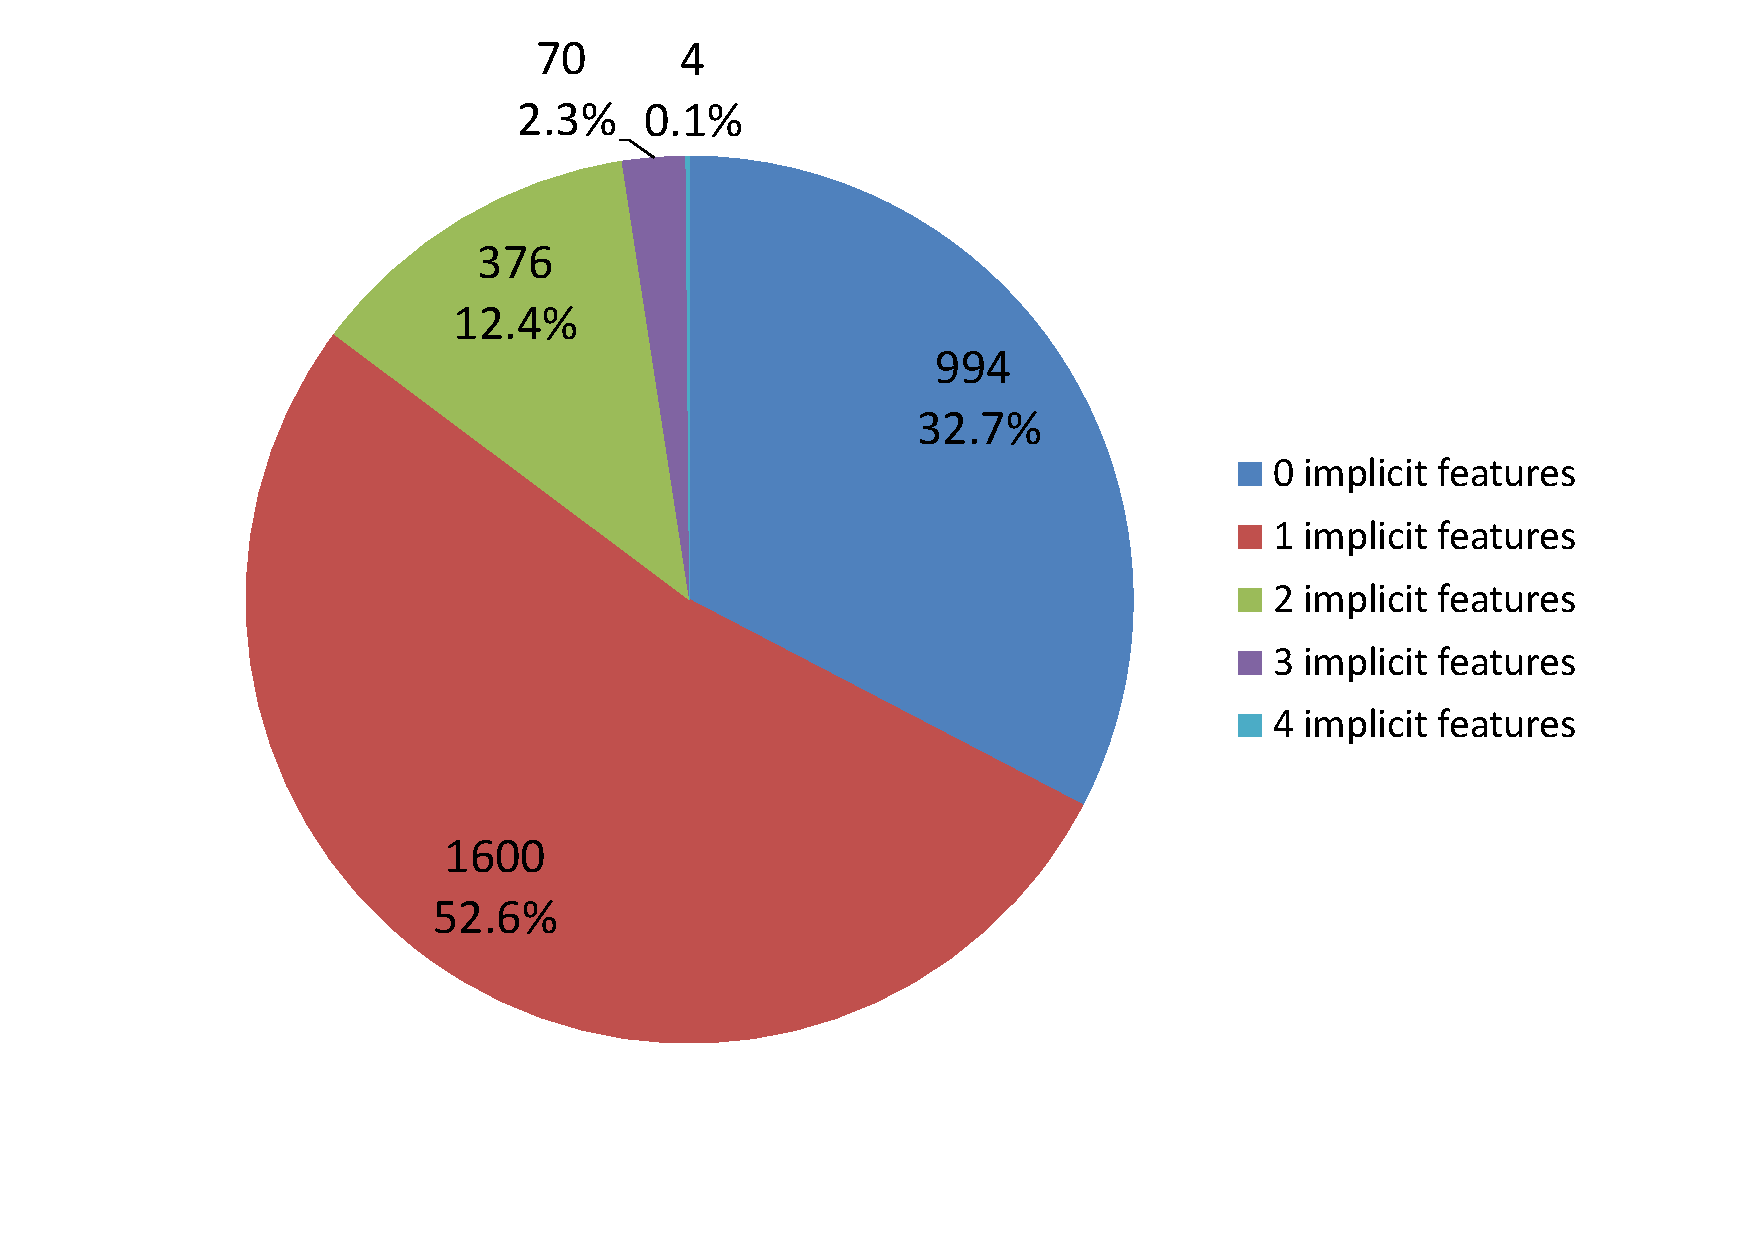
\includegraphics[width=1.4\linewidth]{piechart.pdf}
			\vspace{-22pt}
			\caption{Distribution of the number of implicit features contained per sentence, in the restaurant review data set.}
			\label{fig:piechart}
			
		\end{subfigure}
		\hspace{10pt}
		\begin{subfigure}{.45\textwidth}
			\vspace{38pt}
			\hspace{-20pt}
			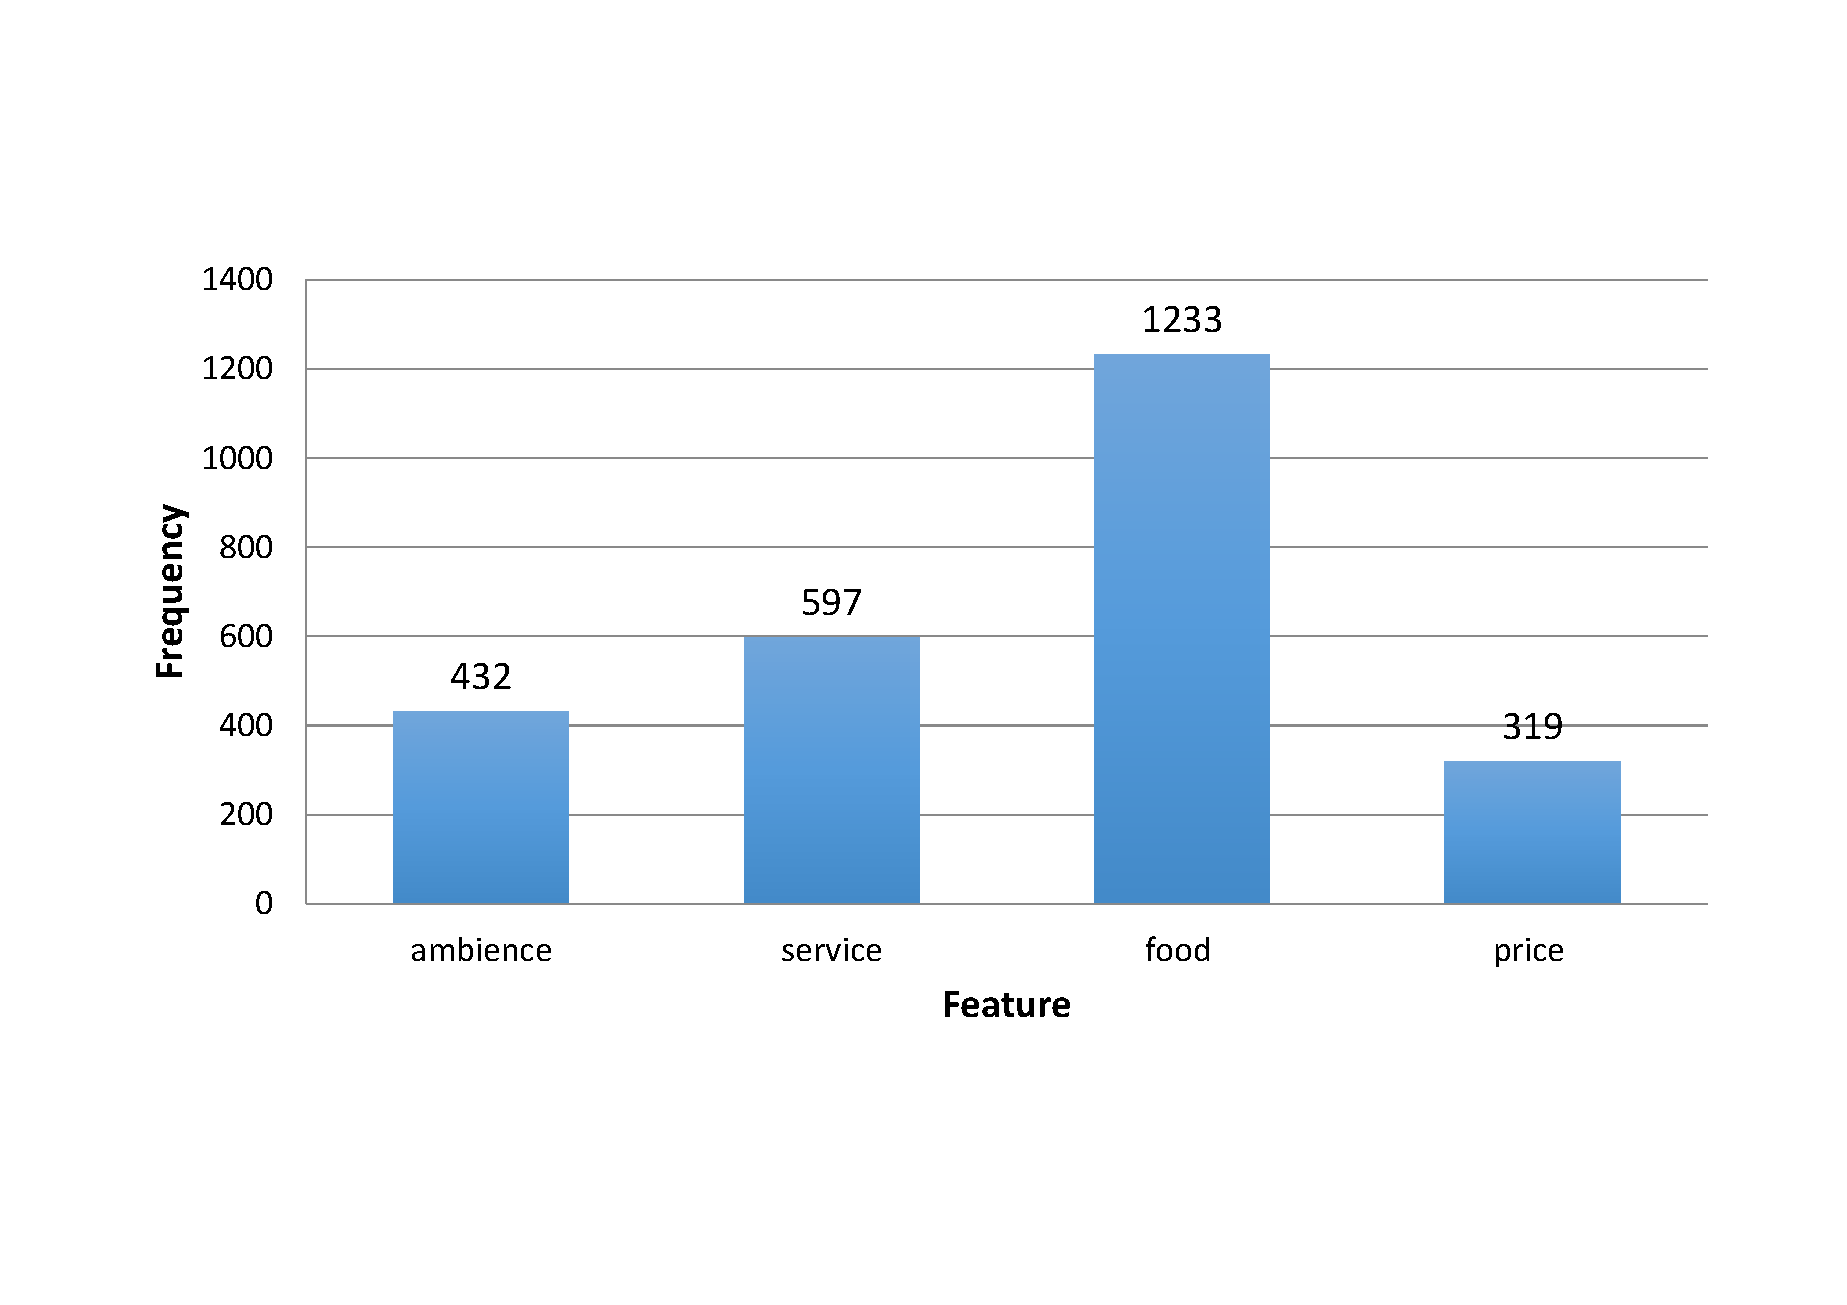
\includegraphics[trim= 20 100 20 100, clip, width=1.2\linewidth]{barchart.pdf}
			\caption{Frequencies of the four unique implicit features in our data set.}
			\label{fig:barcart}
		\end{subfigure}
		\end{center}
		\vspace{-10pt}
	\end{figure}
	
	
	The data set which is used to build up and validate the method proposed in the previous section consists of a collection of restaurants reviews~\cite{GEM2009}. Every review sentence is assigned to at least one of five so-called review aspect categories: `food', `service', `ambience', `price', and `anecdotes/miscellaneous'. These aspect categories are generally not explicitly referred to in a sentence but can be inferred from each sentence. Therefore, these aspect categories operate as \textit{implicit} features of the product, i.e., the restaurant. In the data set, both implicit and explicit restaurant features are labeled. %We note that because there are only five different implicit features, a relatively good performance can be obtained compared to consumer review data sets in which the feature detection algorithm selects from a larger domain \cite{SF2014,ZZ2013}.
	

		
	
	All 3,044 sentences in the restaurant data set contain at least one implicit feature. However, in order to obtain a better performance test of our classifier for the number of implicit features present in each sentence, the fifth category of `anecdotes/miscellaneous' is removed from the data set. This particular category seems most appropriate for removal, as it does not describe a unique implicit feature but refers to the general context `miscellaneous'. In this way, the number of implicit features in our data set has a wider distribution because part of the set now consists of sentences without an implicit feature. As consumer review sentences generally do not always contain an implicit feature, the performance of our classifier on this more realistic scenario is interesting. Furthermore, in this setting the influence of the threshold parameter in the algorithm by~\cite{SF2014} in combination with our classifier can be measured.
	
	\begin{figure}[t]
	\centering
	\scalebox{1}[0.80]{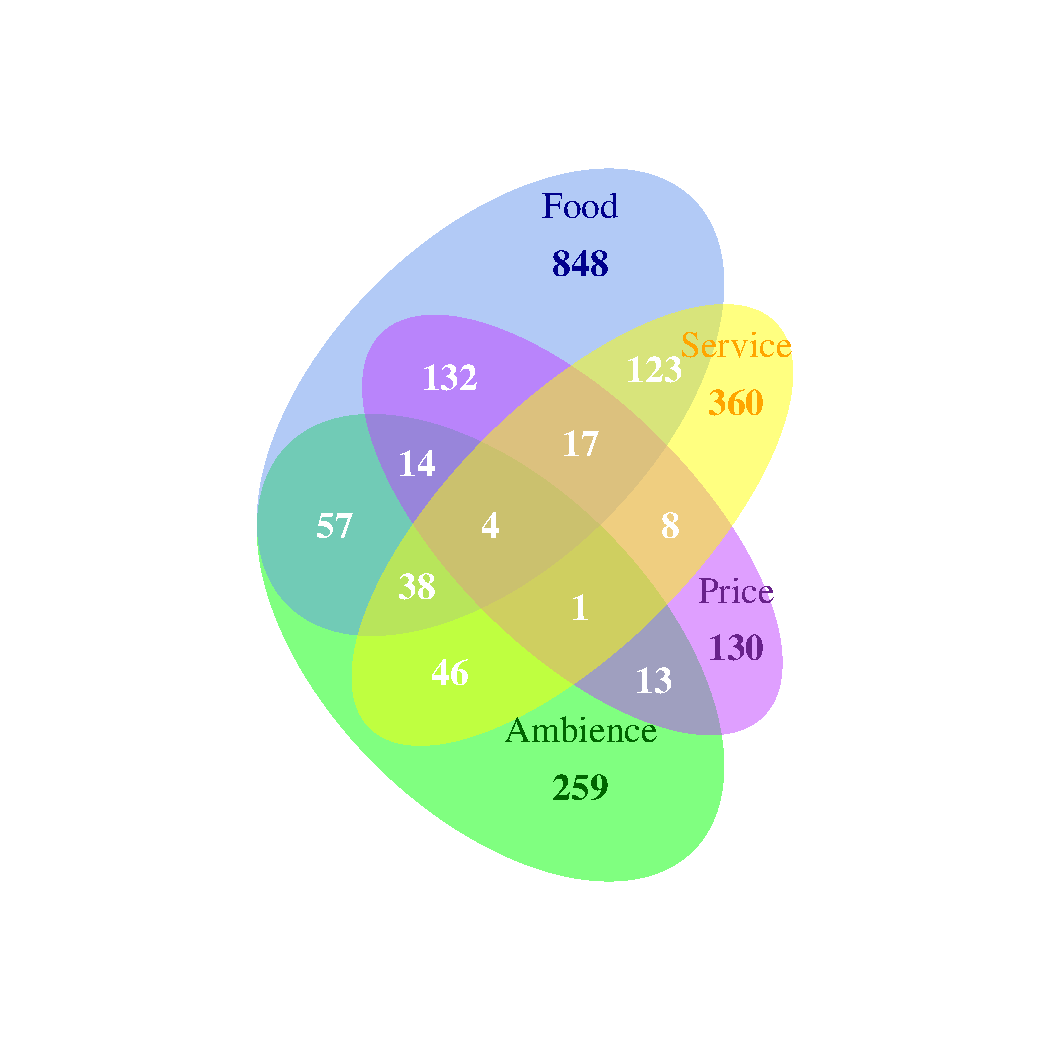
\includegraphics[trim= 40 60 40 80, clip, width=0.8\linewidth]{venn.pdf}}
	\caption{Co-occurrence frequencies of the four unique implicit features in our data set.}
	\label{fig:venn}
	\end{figure}
	
	As clearly displayed in \autoref{fig:piechart}, more than half of the sentences contain only one implicit feature. However, in a significant percentage of sentences, namely 12.4\%, two implicit features are mentioned. This motivates an approach that considers more than one implicit feature in a sentence. %To illustrate this, we provide the following example review:
	
%	\begin{quote}
%	``All of the pizzas are terrific and it's even better that they are so cheap!''
%	\end{quote}	
%	This review contains two implicit features: `food' and `price'. Our method aims to detect both of these features.

	

	Examining the frequency of the four implicit features in \autoref{fig:barcart}, it is clear that all of them play an important role in customer's reviews. Interesting is the fact that each of them appears in more than 300 sentences which is because there is only a small set of features. More specifically, `food' captures more than one third of the sentences in total and more than twice of any of the other categories. In terms of frequency, `food' is followed by the feature `service' appearing in nearly half as many sentences as `food'. Feature `ambience' is implicitly referred to in 432 sentences. Lastly, the least common feature is `price', where the difference with `food' is a factor of three.
	
	
	As the main purpose of the method that we propose is to search for multiple implicit features in each sentence, it seems worthwhile to examine to what extent multiple features are present in one sentence. \autoref{fig:venn} shows the frequency of all possible co-occurrences between the four unique implicit features. Clearly, most of the sentences in our data contain only one implicit feature, something that can also be seen in \autoref{fig:piechart}. More than 4\% of the sentences implicitly refer to both `food' and `price', and almost the same percentage corresponds to the co-occurrence of `food' and `service'. The remaining combinations of two implicit features appear less frequently in the same sentence in our restaurant review data set. %For instance, `service' and `ambience' only co-occur in approximately 1.5\% of the sentences. Remarkably, in 38 sentences `food', `ambience',and `service' are all implied in only one sentence. Finally, in four sentences all four unique features are present.

\section{Implementation}\label{sec:impl}
	
	 To predict the presence of multiple implicit features, we use the score function as given in Eq.~\ref{eq:scoreclassifier}. We think of this score function as a general rule for categorized review data such as our restaurant review data set. In order to specify the correct score function, however, sufficient amount of this type of consumer review data is required. Constrained by resources, however, only the same restaurant review data set is available to us. Therefore, the score function is not trained on a training part of the data set, and then tested on a test part. Instead, the full data set is used in order to maximize the information available to us.
	
	 We estimate the $\mathit{Score}_{k_s}$ function~\eqref{eq:scoreclassifier} using logistic regression. \autoref{tab:coef_reg} displays the results. The $p$-values indicate that our variables are highly significant, i.e., for significance levels below 1\%. Apart from the variables that we include, we also test implementing the number of words in a sentence and the number of grammatical subjects in a sentence. Neither of these variables yield a significant improvement. Intuitively, this can be explained because the variables for the number of nouns and adjectives already capture the relevant information that lies within the number of words within a sentence. The number of subjects possibly does not perform better than the number of nouns because often the subject in a sentence is the product instead of the feature. %For illustration, we provide the following example review:
%	 \begin{quote}
%	 ``The restaurant has a great atmosphere and an amazing staff.''
%	 \end{quote}
	
%	The \textit{subject} in this sentence is `restaurant', which is the reviewed product. However, the \textit{nouns} `atmosphere' and `staff' link to the implicit features `ambience' and `service'.
	
	 \begin{table}[t]
		 \caption{Coefficients of logistic regression \eqref{eq:scoreclassifier} for the classifier.}
		 \label{tab:coef_reg}
		 \centering\vspace{2ex}
	\begin{tabular*}{\textwidth}{@{\extracolsep{\fill}}ldb}
			 \toprule
			 Predictor Variable & \multicolumn{1}{c}{Coefficient} & \multicolumn{1}{c}{$p$-value} \\ \midrule
			 \texttt{Constant} & -3.019479 & 0.0000 \\
			 $\texttt{\#NN}_s$ & 0.116899 & 0.0002 \\
			 $\texttt{\#JJ}_s$ & 0.335530 & 0.0000 \\
			 $\texttt{Comma}_s$ & 0.216417 & 0.0004  \\
			 $\texttt{And}_s$ & 0.399415 & 0.0000  \\\bottomrule	
		 \end{tabular*}
	 \end{table}
	
	The regression is performed on the complete restaurant data set, as motivated above. However, one could argue that this could result in unfair performance, as the same data set is used to evaluate our algorithm. However, when the coefficients of the regression are robust for different subsamples, specifying a different score function based on an arbitrary train part of the data set will not alter the results heavily. Put differently, this would indicate that our approach of using the full data set does not provide an unfair edge. To check whether this is the case, we perform the logistic regression 1000 times on arbitrary subsamples containing 90\% of the data set. \autoref{fig:box_var} depicts the coefficients of the 1000 regressions in a box-plot and \autoref{tab:coef_reg_1000} provides descriptive statistics. The constant is excluded from the plot and table, because it does not influence the result with a trained threshold. We find that the values of the coefficients do not differ a lot for the different subsamples, so it is justified to use the complete data set when determining the coefficients. % We note that as the coefficients are highly significant for the full data set, we may fairly say that all coefficients for the different subsamples are also significant without further investigation.
		
	\begin{table}[t]
			 \caption{Specifications of 1000 logistic regressions on 90\% subsamples.}
			 \label{tab:coef_reg_1000}
			 \vspace{2ex}
			 \centering
	\begin{tabular*}{\textwidth}{@{\extracolsep{\fill}}ldbd}
				 \toprule
				 Variable &\multicolumn{1}{c}{Mean} & \multicolumn{1}{c}{Median} & \multicolumn{1}{c}{Std. dev.} \\ \midrule
				 $\texttt{\#NN}_s$ & 0.117361 & 0.11768 & 0.011342 \\
				 $\texttt{\#JJ}_s$ & 0.335538 & 0.33536 & 0.014345 \\
				 $\texttt{Comma}_s$ & 0.216409 & 0.21672 & 0.023185 \\
				 $\texttt{And}_s$ & 0.399507 & 0.39892 & 0.023409 \\	 \bottomrule
			 \end{tabular*}
		 \end{table}

	\begin{figure}[t]
		\centering
		\vspace{-10pt}
		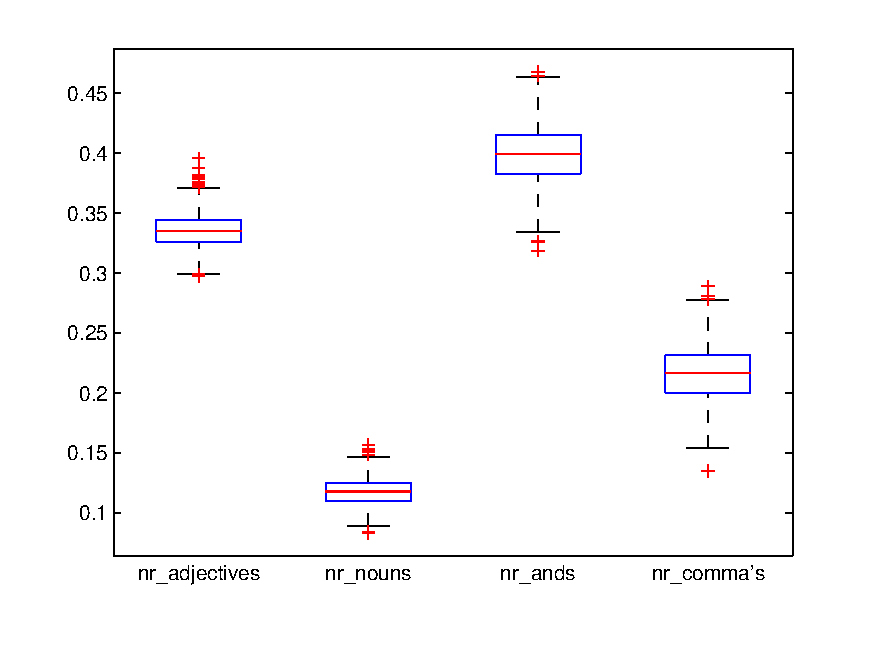
\includegraphics[width=0.8\linewidth]{boxplot_variables.pdf}
		\vspace{-12pt}
		\caption{Box-plot of the coefficients of the logistic regression.}
		\label{fig:box_var}
	\end{figure}
	

	
	The classifier predicts multiple implicit features for sentence $s$ when $\text{Score}_{k_s}$ is larger than a certain threshold. We can therefore train the classifier by determining the optimal threshold. In order to do so, we isolate the performance of the classifier by assuming that the feature detection part of the algorithm is perfect. That is, if the classifier predicts the presence of multiple implicit features correctly, we assign all golden implicit features to that sentence; if the classifier predicts incorrectly, we assign either only one golden implicit feature (in case there are actually multiple implicit features), or one implicit feature too many (in case there are not actually multiple features) to the sentence. This way, the errors made by the classifier are isolated and can thus be minimized by means of altering the threshold.
	
	%Now, the performance of the classifier (with a certain threshold) is evaluated with an $\textit{F}_{\beta}$-score.  This performance measure, which is taken from the effectiveness measure that is introduced in \cite{R1979}, is one of the standard measures within the feature detection literature. The $\textit{F}_{\beta}$-score is defined as follows:
				
%	\begin{align}\label{eq:F_beta_algorithm}
%		{F_\beta} = (1+\beta^2)\cdot\frac{\mathit{precision} \cdot \mathit{recall}}{(\beta^2 \cdot \mathit{precision}) + \mathit{recall}},
%	\end{align}			
%	for $\beta>0$. \textit{Precision} is the percentage following from dividing the number of correctly predicted implicit features by the total amount of implicit features that are predicted. \textit{Recall} is the percentage obtained by dividing the number of correctly predicted implicit features by the amount of implicit features that should have been predicted. The scaling factor $\beta$ gives a higher relative weight to either precision or recall. If $\beta$ is set equal to 1, precision and recall are considered equally important. For $\beta<1$, precision obtains a relatively higher weight and for $\beta>1$ recall can be considered more important.

	The classifier is optimized on $\textit{F}_{\beta}$-score. Since the main goal of our classifier is to predict multiple implicit features when they are present, high recall is especially important. If it incorrectly predicts no multiple implicit features in the sentence, the recall of the final score will always decrease, because there can only be one implicit feature assigned to that sentence. However, when the classifier incorrectly predicts the presence of multiple implicit features, the precision of the final score does not necessarily decrease. The threshold in the feature detection part of the algorithm could prevent that multiple implicit features are assigned to a sentence. %Therefore, recall is relatively more important than precision, when evaluating the classifier.
	\autoref{fig:beta_rec_prec} shows the precision and recall of the classifier with a trained threshold for different $\beta$'s. It can be seen that with $\beta$ larger than 1.8, the precision decreases relatively fast, while the recall only increases a little bit. Therefore, we use $\beta$ equal to 1.8 in the $F_\beta$-score when training the classifier to emphasize recall.
	
	\begin{figure}[t]
			\centering
			\vspace{-25pt}
			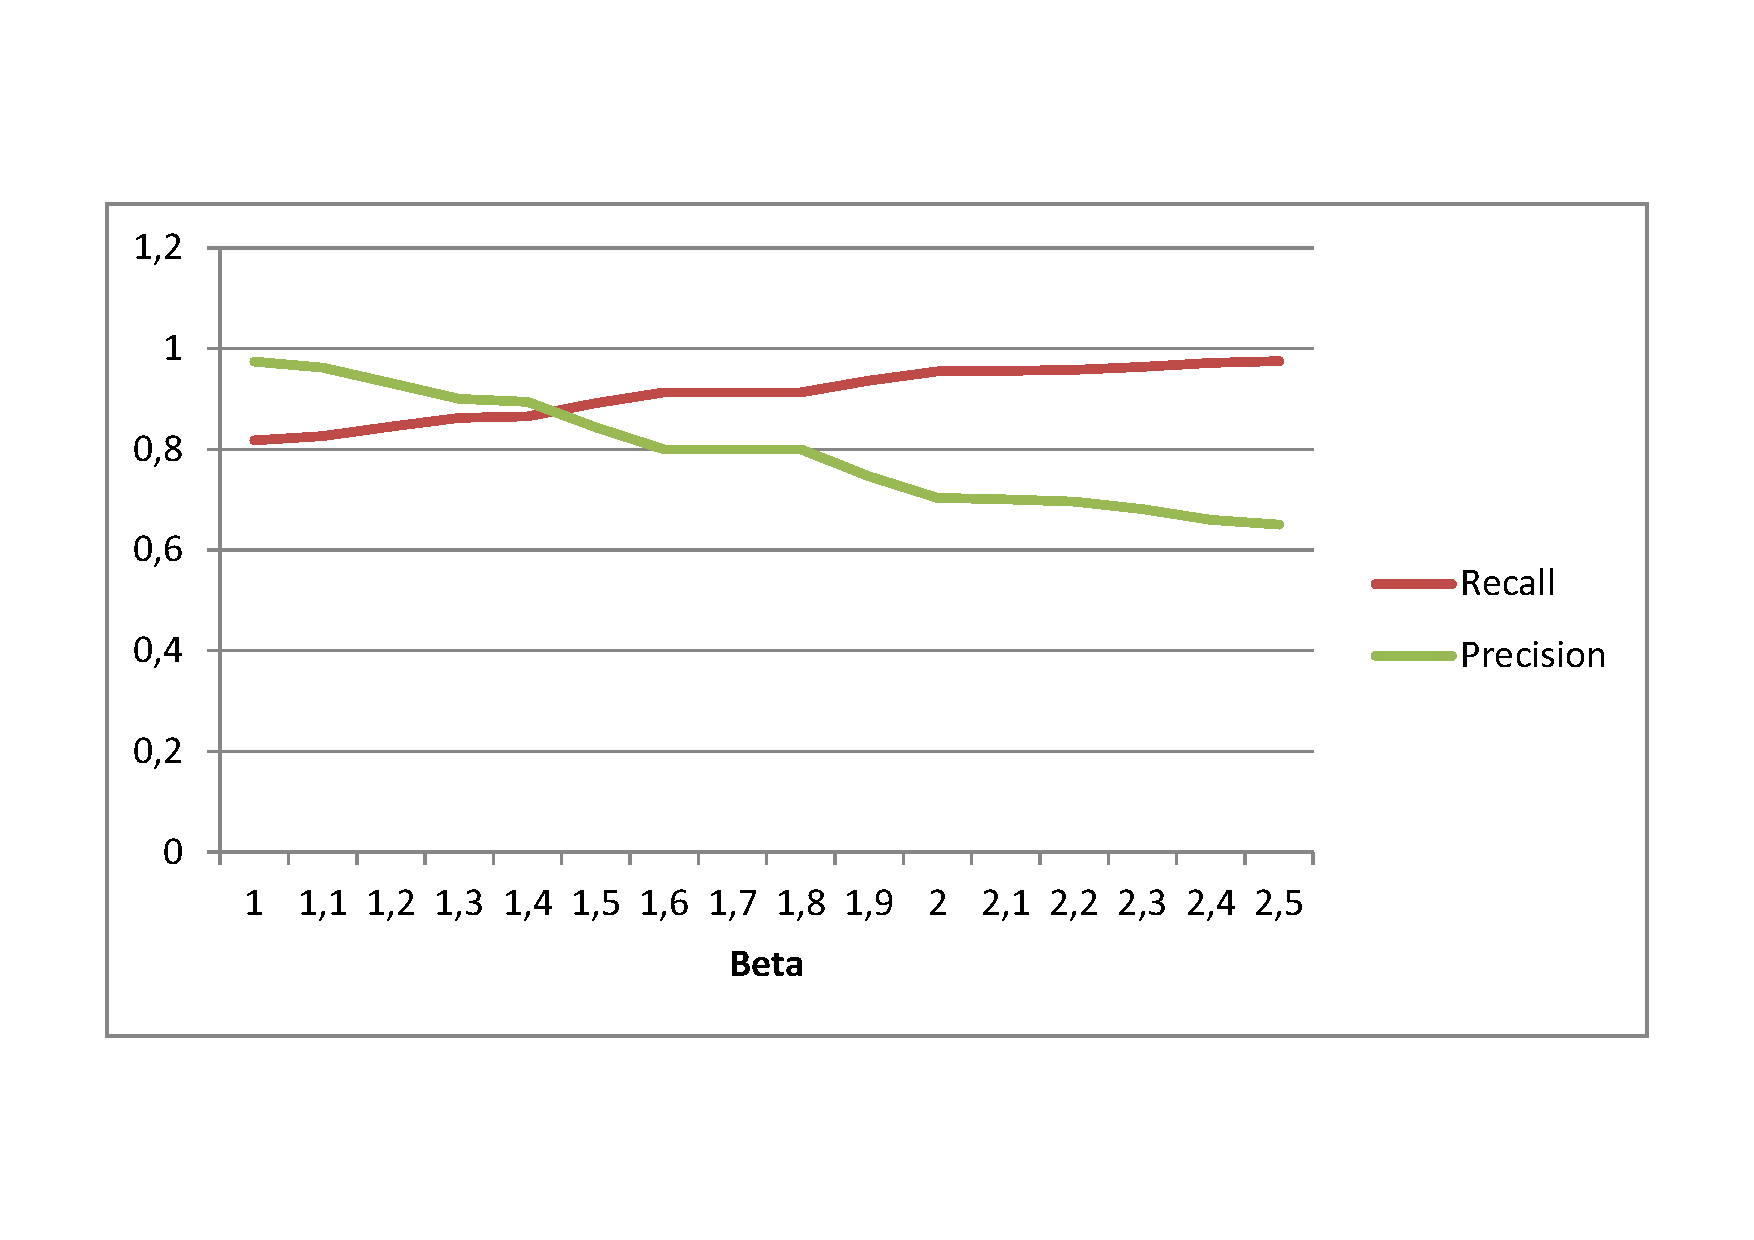
\includegraphics[trim= 65 101 65 100, clip, width=\linewidth]{beta_recall_precision.pdf}
			\vspace{-12pt}
			\caption{Recall and precision of the classifier for different $\beta$'s.}
			\label{fig:beta_rec_prec}
	\end{figure}
	
	 Finally, the threshold is trained on an annotated training set containing 90\% of the data. To train the threshold, a range of threshold values needs to be defined. We use values between $-3$ and 3, with a step size of 0.1. With every threshold, the classifier is evaluated based on $F_{1.8}$. Hence, after linearly trying all possible thresholds, we use the threshold with the largest $\text{F}_{1.8}$-score.

\section{Evaluation}\label{sec:eval}
	Evaluation of the implemented method is based on 10-fold cross-evaluation. This means that the whole data set is split into two subsets: one part contains 90\% of the data, the other part 10\%. The algorithm is then trained on this 90\% of the data set. The trained algorithm then detects the implicit features in the remaining 10\% of the data. This procedure is repeated 10 times, where there is no overlap in the 10 hold-out samples. For each fold, the $F_1$-score is calculated and finally averaged to provide the measure for the performance of the algorithm.
	

	
	The predictive performance we consider to evaluate the predicting of implicit features is the $F_1$-score %, which is the $\textit{F}_{\beta}$-score as given in \eqref{eq:F_beta_algorithm}, with $\beta$ = 1
	. Using the $F_1$-score as the performance measure allows for easy comparison with previous work, as it is one of the standard performance measures within the literature. %However, we note that for other than academic purposes, choosing a $\beta$ equal to 1 is not necessarily the optimal choice for any feature detection project.
		
	Because the different  training and test subsamples used in the cross-evaluation are generated randomly, we run our algorithm 10 times. \autoref{fig:pos_mean} shows the results, in terms of mean $F_1$-scores, following from our proposed method (the blue bars). To provide more insights into our results, \autoref{fig:pos_mean} also depicts $F_1$-scores of the algorithm with both a perfect classifier (the red line) and with a perfect feature detection algorithm (the green line). The scores using a perfect classifier are computed by always passing the correct prediction (in terms of the presence of multiple implicit features) onto the feature detection algorithm.  The scores with the perfect feature detection are found by, based on the prediction of the classifier, assigning a number of golden implicit features to the sentences.
	
	Results are given for different part-of-speech filters, which are used to filter out possibly irrelevant words in the co-occurrence matrix that could be harmful to the performance of the algorithm. \autoref{fig:pos_mean} shows the scores for 16 different part-of-speech filters. The filters include only the words of types that are mentioned, where \texttt{NN} stands for nouns, \texttt{VB} for verbs, \texttt{JJ}, for adjectives and \texttt{RB} for adverbs.
	Examining the $F_1$-scores in \autoref{fig:pos_mean}, we find that the best results are obtained using the \texttt{NN+JJ} part-of-speech filter. That is, filtering for nouns and adjectives, we obtain an $F_1$-score equal to $64.5\%$. We note that the $F_1$-score we find for using the \texttt{NN} filter is only marginally worse, namely 64.1\%.
	
			\begin{figure}[t]
					\centering
					\vspace{-25pt}
					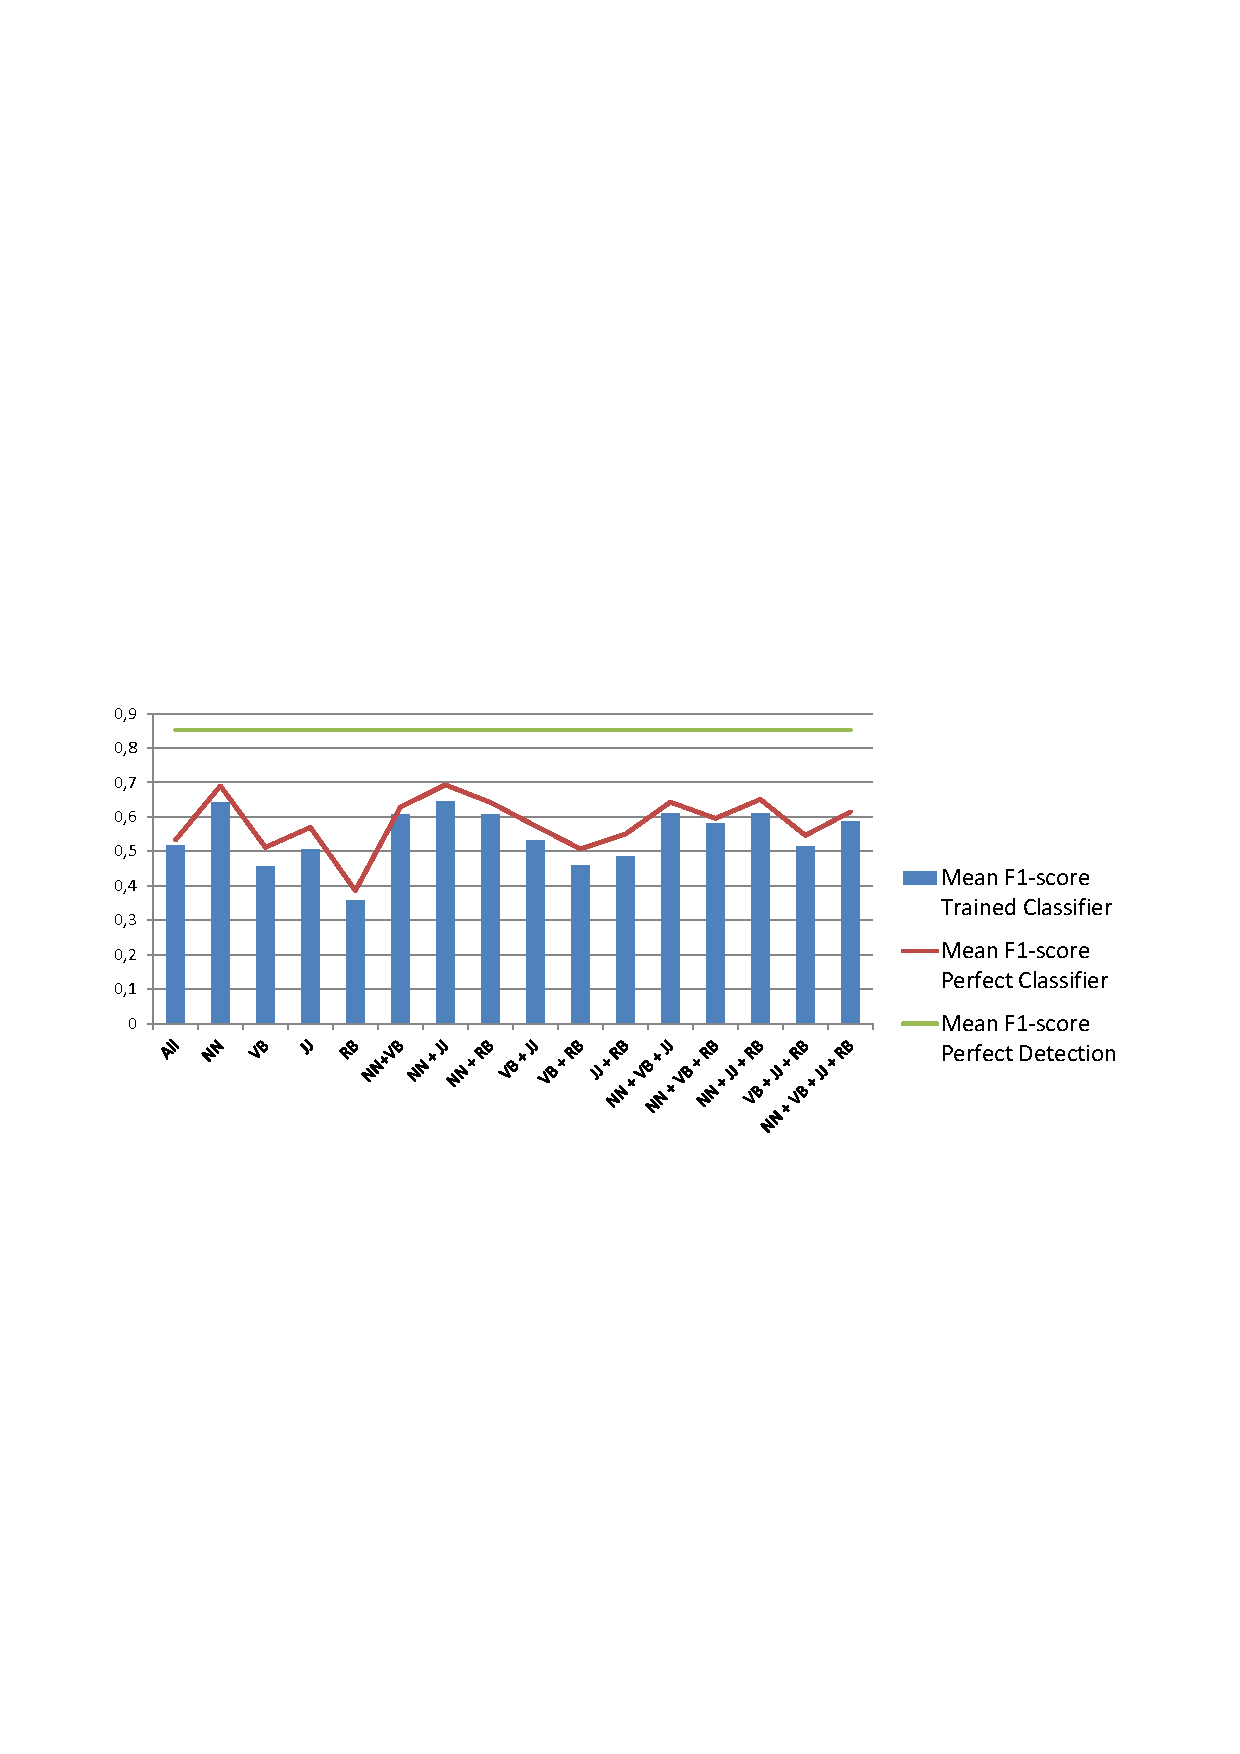
\includegraphics[trim= 55 277 55 320, clip, width=\linewidth]{POS_mean.pdf}
					\vspace{-12pt}
					\caption{Mean $F_1$-scores with different part-of-speech filters.}
					\label{fig:pos_mean}
			\end{figure}
	
	Since our proposed method extends the one presented in~\cite{SF2014}, we start by evaluating the increase in performance as a result of our extension. In order to do so, we also evaluate the unextended algorithm as presented in~\cite{SF2014} 10 times using the \texttt{NN+JJ} part-of-speech filter. Again, we note that each evaluation provides slightly different results due to the random nature of the cross-evaluation method. We find a mean $F_1$-score of $62.9\%$ for the algorithm without the classifier.\footnote{We note that in~\cite{SF2014}, based on a number of runs, a maximum $F_1$-score of 63.3\% is reported.} Hence, comparing this to our 64.5\%, we find an improvement of 1.6 percentage points. We test for significance by means of a two-sample $t$-test. This results in a $t$-test statistic equal to $12.0$, which indicates a significant improvement at the significance level of 1\%. 	
	
	At first sight, an improvement in mean $F_1$-score of 1.6 percentage points may not look large. However, in order to make a fair statement about the performance of our classifier, we first need to compare it to its potential, which is displayed by the red line in \autoref{fig:pos_mean}. We see that the potential is also at its largest for the \texttt{NN+JJ} filter, giving an $F_1$-score of 69.3\%.  This means that our classifier captures 25\% of the maximum improvement that can be gained by adding a classifier that predicts the presence of multiple implicit features within a sentence, which is 6.4\%.  However, we note that the potential of such a classifier depends on the data set. In our restaurant review data set, 14.8\% of the sentences contain more than one implicit feature, where 12.4\% of the sentences contain two implicit features. Furthermore, calculations show that 20.4\% of the total possible implicit features  remain to be detected when only one implicit feature per sentence is considered.\footnote{Based on the distribution of the number of implicit features per sentence in our data set (see \autoref{fig:piechart}), we have: $(12.4+2\cdot2.3+3\cdot0.1)/(52.6+2\cdot12.4+3\cdot2.3+4\cdot0.1)=0.204$.} However, it is important to notice that the most apparent implicit feature in each sentence is already detected. As a result, the second implicit feature would be assigned with an already lower precision, tempering the improvement of the $F_1$-score due to a higher recall. Therefore, in light of these insights and considering the simplicity of our approach, we consider our gained improvement to be significant.
	
	Lastly, we provide insights in our results by looking at the $F_1$-score that can be obtained by using our classifier in combination with a perfect feature detection algorithm, which is displayed by the green line in \autoref{fig:pos_mean}. Notice that our classifier is trained to maximize the $\textit{F}_{1.8}$-score. For this reason, these `potential' $F_1$-scores are hardly interpretable and a greater potential might be visible when the classifier is trained for the same measure by which it is now evaluated. However, training for $F_{1.8}$ yields best \textit{overall} performance in our method, which is also motivated in Sect.~\ref{sec:impl}. Nonetheless, these $F_1$-scores provide insight in what part in the loss of $F_1$-score can be attributed to the feature detection part of our algorithm. The $F_1$-scores with perfect detection, which do not rely on the part-of-speech filters, are $85.2\%$. Comparing this result with the one in the previous paragraph, we conclude that improving the feature detection part of the algorithm shows greater potential than improving the prediction of the presence of multiple implicit features.
	

	

	

	
	


\section{Conclusion}\label{sec:conc}
	In many of the existing methods within the literature, detection algorithms are limited to assigning only one implicit feature per sentence. However, when consumers review their purchased products, they do typically not obey this constraint. Therefore, based on this visible shortcoming in previous work, we propose an algorithm that allows for the detection of multiple implicit features per sentence. Our method directly extends the more constrained, supervised method earlier proposed in~\cite{SF2014}.
	
	In our proposed method we construct a classifier that predicts the presence of multiple implicit features using a score function. The score function is based on four simple sentence characteristics: (i) number of nouns, (ii) number of adjectives, (iii) number of commas, and (iv) the number of `and' words. The function parameters are estimated by means of logistic regression and we train a threshold for better performance. Based on the prediction of the classifier for a given review, the feature detection part of our algorithm then looks for either one or multiple implicit features.
	
	Considered on a restaurant review data set, our approach shows small but significant improvement with respect to the constrained method in~\cite{SF2014}. That is, we improve the $F_1$-measure by 1.6 percentage points. Based on analysis of the performance of our classifier we conclude that we capture a reasonable (considering its simplicity) part of the full potential of our approach. The performance and potential of the classifier is however dependent on the distribution of the number of implicit features per sentence within the data set. That is, when consumer reviews frequently cover multiple implicit features per sentence, our more realistic approach is desirable.
	
	In our approach we determine a \textit{general} relation between sentences written in consumer reviews and the number of implicit features. Nonetheless, it might be desirable to integrate the specification and estimation of this relation in the training part of the algorithm in order to make it specifically effective for a given data set.	One promising path for future work is therefore to train a classifier for the number of implicit features by using more advanced machine-learning techniques, such as Support Vector Machines. Also, rule learning methods could be employed in order to determine more indicators for the presence of multiple implicit features.	
	
	Another interesting suggestion for future research may be to combine the classifier with sentiment analysis algorithms. Namely, when there are opposing sentiments within one sentence, it seems likely that the consumer is commenting on two different features of the product. To illustrate this idea, we provide the following example:
	\begin{quote}
	``The phone looks great, but the pictures it takes are of very low quality.''
	\end{quote}
	In this sentence, two features are implied: `appearance' and 'camera'. Also, there are two sentiment polarities: the consumer is positive about the appearance, but negative about the camera. %While simply detecting for both negative and positive polarities seems promising, one could use the distance between pairs of scaled sentiments within one sentence as an indicator for the presence of multiple implicit features. For the latter, more sophisticated sentiment extraction methods are required.
	
	
	

\section*{Acknowledgments}
	The authors are partially supported by the Dutch national program COMMIT.
%	We thank Flavius Frasincar for his friendly assistance and helpful remarks. We particularly thank Kim Schouten for sharing his framework and contributions to our work.

\bibliographystyle{splncs03}
\bibliography{sources}

\end{document}
